%\RequirePackage[l2tabu, orthodox]{nag}
\RequirePackage{currfile}
\documentclass[12pt]{beamer}
\graphicspath{{Imagenes/}{../Imagenes/}}
\usepackage[utf8]{inputenc}
\usepackage[spanish]{babel}
\usepackage{standalone}
\usepackage{color}
\usepackage[binary-units=true]{siunitx}
\usepackage{hyperref}
\hypersetup{
  colorlinks=true,
  linkcolor=blue,          % color of internal links (change box color with linkbordercolor)
  citecolor=green,        % color of links to bibliography
  filecolor=magenta,      % color of file links
  urlcolor=cyan,           % color of external links
  linkbordercolor={0 0 1}
}
\usepackage{xcolor, soul}
\usepackage{etoolbox}
\usepackage{amsmath}
\usepackage{amsthm}
\usepackage{physics}
\usepackage{multicol}
\usepackage{graphicx}
\usepackage{bookmark}
\usepackage{longtable}
\usepackage{graphicx}
\usepackage{tikz}
\usepackage[siunitx, RPvoltages]{circuitikz}
\usetikzlibrary{mindmap}
\usetikzlibrary{arrows, patterns, shapes, decorations.markings, decorations.pathmorphing}
\usetikzlibrary{matrix,positioning}
\tikzstyle{every picture}+=[remember picture,baseline]
\usepackage[autostyle,spanish=mexican]{csquotes}
\usepackage{pifont}
\usepackage[font=footnotesize,textfont=it]{caption}
\usepackage{tabulary}
\usepackage{booktabs}
\usepackage[outdir=./]{epstopdf}
%\usepackage{epstopdf}
\usepackage{media9}
\usepackage{multimedia}
\usepackage{bigints}
%\usepackage{enumitem}
\usepackage[os=win]{menukeys}
\usepackage{pifont}
\usepackage{pbox}
\usepackage{alltt}
\usepackage{verbatim}
\usepackage{colortbl}
\usepackage{tcolorbox}
\usepackage{fancyvrb}
\usepackage[sfdefault]{roboto}  %% Option 'sfdefault' only if the base font of the document is to be sans serif
%\usepackage[T1]{fontenc}
\setcounter{secnumdepth}{3}
\setcounter{tocdepth}{3}
\DeclareGraphicsExtensions{.pdf,.png,.jpg}
\renewcommand {\arraystretch}{1.5}
\definecolor{ao}{rgb}{0.0, 0.5, 0.0}
\definecolor{aquamarine}{rgb}{0.5, 1.0, 0.83}
\definecolor{kellygreen}{rgb}{0.3, 0.73, 0.09}
\definecolor{bisque}{rgb}{1.0, 0.89, 0.77}
\definecolor{amber}{rgb}{1.0, 0.75, 0.0}
\definecolor{armygreen}{rgb}{0.29, 0.33, 0.13}
\definecolor{alizarin}{rgb}{0.82, 0.1, 0.26}
\definecolor{cadetblue}{rgb}{0.37, 0.62, 0.63}
\newcommand*{\TitleParbox}[1]{\parbox[c]{6cm}{\raggedright #1}}%
\newcommand{\python}{\texttt{python}}
\newcommand{\textoazul}[1]{\textcolor{blue}{#1}}
\newcommand{\azulfuerte}[1]{\textcolor{blue}{\textbf{#1}}}
\newcommand{\funcionazul}[1]{\textcolor{blue}{\textbf{\texttt{#1}}}}
%\normalfont
\usepackage{ccfonts}% http://ctan.org/pkg/{ccfonts}
\usepackage[T1]{fontenc}% http://ctan.or/pkg/fontenc
\renewcommand{\rmdefault}{cmr}% cmr = Computer Modern Roman
\usefonttheme[onlymath]{serif}
\linespread{1.3}
\newcounter{saveenumi}
\newcommand{\seti}{\setcounter{saveenumi}{\value{enumi}}}
\newcommand{\conti}{\setcounter{enumi}{\value{saveenumi}}}
\newcommand{\tikzmark}[1]{\tikz[remember picture] \node[coordinate] (#1) {#1};}

\usepackage{scalerel}[2016-12-29]
\def\stretchint#1{\vcenter{\hbox{\stretchto[440]{\displaystyle\int}{#1}}}}
\def\scaleint#1{\vcenter{\hbox{\scaleto[3ex]{\displaystyle\int}{#1}}}}
\def\bs{\mkern-12mu}

\newtheorem{teo}{}[section]
\usepackage{blkarray}

%reduce el tamaño de letra de la etiqueta equations
\makeatletter
\def\maketag@@@#1{\hbox{\m@th\normalfont\small#1}}
\makeatother

%se usa para la x en itemize
\newcommand{\xmark}{\text{\ding{55}}}

%\AtBeginDocument{\setlength{\tymin}{1em}}


\definecolor{myblue}{rgb}{.8, .8, 1}

\usepackage{empheq}

\newlength\mytemplen
\newsavebox\mytempbox

\makeatletter
\newcommand\mybluebox{%
    \@ifnextchar[%]
       {\@mybluebox}%
       {\@mybluebox[0pt]}}

\def\@mybluebox[#1]{%
    \@ifnextchar[%]
       {\@@mybluebox[#1]}%
       {\@@mybluebox[#1][0pt]}}

\def\@@mybluebox[#1][#2]#3{
    \sbox\mytempbox{#3}%
    \mytemplen\ht\mytempbox
    \advance\mytemplen #1\relax
    \ht\mytempbox\mytemplen
    \mytemplen\dp\mytempbox
    \advance\mytemplen #2\relax
    \dp\mytempbox\mytemplen
    \colorbox{myblue}{\hspace{1em}\usebox{\mytempbox}\hspace{1em}}}

\makeatother



%Se usa la plantilla Madrid modificada con beaver
\mode<presentation>
{
  \usetheme{Madrid}
  \setbeamertemplate{headline}{}
  %\useoutertheme{infolines}
  \usecolortheme{beaver}
  \setbeamercovered{invisible}
  

\setbeamertemplate{section in toc}[sections numbered]
\setbeamertemplate{subsection in toc}[subsections numbered]
\setbeamertemplate{subsection in toc}{\leavevmode\leftskip=3.2em\rlap{\hskip-2em\inserttocsectionnumber.\inserttocsubsectionnumber}\inserttocsubsection\par}
\setbeamercolor{section in toc}{fg=blue}
\setbeamercolor{subsection in toc}{fg=blue}
\setbeamerfont{subsection in toc}{size=\small}

\setbeamertemplate{navigation symbols}{}
\setbeamertemplate{caption}[numbered]

}

\usepackage{courier}
\usepackage{listingsutf8}
\usepackage{listings}
\usepackage{xcolor}
\usepackage{textcomp}
\usepackage{color}
\definecolor{deepblue}{rgb}{0,0,0.5}
\definecolor{brown}{rgb}{0.59, 0.29, 0.0}
\definecolor{OliveGreen}{rgb}{0,0.25,0}
% \usepackage{minted}

\DeclareCaptionFont{white}{\color{white}}
\DeclareCaptionFormat{listing}{\colorbox{gray}{\parbox{0.98\textwidth}{#1#2#3}}}
\captionsetup[lstlisting]{format=listing,labelfont=white,textfont=white}
\renewcommand{\lstlistingname}{Código}


\definecolor{Code}{rgb}{0,0,0}
\definecolor{Keywords}{rgb}{255,0,0}
\definecolor{Strings}{rgb}{255,0,255}
\definecolor{Comments}{rgb}{0,0,255}
\definecolor{Numbers}{rgb}{255,128,0}

\makeatletter

\newif\iffirstchar\firstchartrue
\newif\ifstartedbyadigit
\newif\ifprecededbyequalsign

\newcommand\processletter
{%
  \ifnum\lst@mode=\lst@Pmode%
    \iffirstchar%
        \global\startedbyadigitfalse%
      \fi
      \global\firstcharfalse%
    \fi
}

\newcommand\processdigit
{%
  \ifnum\lst@mode=\lst@Pmode%
      \iffirstchar%
        \global\startedbyadigittrue%
      \fi
      \global\firstcharfalse%
  \fi
}

\lst@AddToHook{OutputOther}%
{%
  \lst@IfLastOtherOneOf{=}
    {\global\precededbyequalsigntrue}
    {}%
}

\lst@AddToHook{Output}%
{%
  \ifprecededbyequalsign%
      \ifstartedbyadigit%
        \def\lst@thestyle{\color{orange}}%
      \fi
    \fi
  \global\firstchartrue%
  \global\startedbyadigitfalse%
  \global\precededbyequalsignfalse%
}

\lstset{ 
language=Python,                % choose the language of the code
basicstyle=\footnotesize\ttfamily,       % the size of the fonts that are used for the code
numbers=left,                   % where to put the line-numbers
numberstyle=\scriptsize,      % the size of the fonts that are used for the line-numbers
stepnumber=1,                   % the step between two line-numbers. If it is 1 each line will be numbered
numbersep=5pt,                  % how far the line-numbers are from the code
backgroundcolor=\color{white},  % choose the background color. You must add \usepackage{color}
showspaces=false,               % show spaces adding particular underscores
showstringspaces=false,         % underline spaces within strings
showtabs=false,                 % show tabs within strings adding particular underscores
frame=single,   		% adds a frame around the code
tabsize=2,  		% sets default tabsize to 2 spaces
captionpos=t,   		% sets the caption-position to bottom
breaklines=true,    	% sets automatic line breaking
breakatwhitespace=false,    % sets if automatic breaks should only happen at whitespace
escapeinside={\#},  % if you want to add a comment within your code
stringstyle =\color{OliveGreen},
%otherkeywords={{as}},             % Add keywords here
keywordstyle = \color{blue},
commentstyle = \color{black},
identifierstyle = \color{black},
literate=%
         {á}{{\'a}}1
         {é}{{\'e}}1
         {í}{{\'i}}1
         {ó}{{\'o}}1
         {ú}{{\'u}}1
%
%keywordstyle=\ttb\color{deepblue}
%fancyvrb = true,
}

\lstdefinestyle{FormattedNumber}{%
    literate={0}{{\textcolor{red}{0}}}{1}%
             {1}{{\textcolor{red}{1}}}{1}%
             {2}{{\textcolor{red}{2}}}{1}%
             {3}{{\textcolor{red}{3}}}{1}%
             {4}{{\textcolor{red}{4}}}{1}%
             {5}{{\textcolor{red}{5}}}{1}%
             {6}{{\textcolor{red}{6}}}{1}%
             {7}{{\textcolor{red}{7}}}{1}%
             {8}{{\textcolor{red}{8}}}{1}%
             {9}{{\textcolor{red}{9}}}{1}%
             {.0}{{\textcolor{red}{.0}}}{2}% Following is to ensure that only periods
             {.1}{{\textcolor{red}{.1}}}{2}% followed by a digit are changed.
             {.2}{{\textcolor{red}{.2}}}{2}%
             {.3}{{\textcolor{red}{.3}}}{2}%
             {.4}{{\textcolor{red}{.4}}}{2}%
             {.5}{{\textcolor{red}{.5}}}{2}%
             {.6}{{\textcolor{red}{.6}}}{2}%
             {.7}{{\textcolor{red}{.7}}}{2}%
             {.8}{{\textcolor{red}{.8}}}{2}%
             {.9}{{\textcolor{red}{.9}}}{2}%
             {\ }{{ }}{1}% handle the space
         ,%
          %mathescape=true
          escapeinside={__}
          }



\makeatletter
\setbeamercolor{section in foot}{bg=green!30!cyan, fg=black!90!orange}
\setbeamercolor{subsection in foot}{bg=red!30!cyan, fg=red}
%\setbeamercolor{date in foot}{bg=orange!30!cyan, fg=red}
\setbeamertemplate{footline}
{
  \leavevmode%
  \hbox{%
  \begin{beamercolorbox}[wd=.333333\paperwidth,ht=2.25ex,dp=1ex,center]{section in foot}%
    \usebeamerfont{section in foot} \insertsection
  \end{beamercolorbox}}%
  \begin{beamercolorbox}[wd=.333333\paperwidth,ht=2.25ex,dp=1ex,center]{subsection in foot}%
    \usebeamerfont{subsection in foot}  \insertsubsection
  \end{beamercolorbox}%
  \begin{beamercolorbox}[wd=.333333\paperwidth,ht=2.25ex,dp=1ex,right]{date in head/foot}%
    \usebeamerfont{date in head/foot} \insertshortdate{} \hspace*{2em}
    \insertframenumber{} / \inserttotalframenumber \hspace*{2ex} 
  \end{beamercolorbox}}%
  \vskip0pt%
\makeatother
\title{Integración numérica}
\subtitle{Tema 2 - Operaciones matemáticas básicas}
\author{M. en C. Gustavo Contreras Mayén}
\date{\today}
\institute{Facultad de Ciencias - UNAM}
\titlegraphic{
\includegraphics[width=1.75cm]{Imagenes/escudo-facultad-ciencias}\hspace*{4.75cm}~%
   
\includegraphics[width=1.75cm]{Imagenes/escudo-unam}
}
\begin{document}
\maketitle
\fontsize{14}{14}\selectfont
\spanishdecimal{.}
\section*{Contenido}
\frame{\tableofcontents[currentsection, hideallsubsections]}
\section{Integración numérica}
\frame{\tableofcontents[currentsection, hideothersubsections]}
\subsection{Problema inicial}
\begin{frame}
\frametitle{Problema inicial}
Dada la función $f(x)$, queremos calcular
\[\int_{a}^{b} f(x) dx\]
\end{frame}
\section{Introducción}
\frame{\tableofcontents[currentsection, hideothersubsections]}
\subsection{Base de la integración numérica}
\begin{frame}
\frametitle{Introducción}
La integración numérica (también conocida como \textcolor{blue}{cuadratura}) es un procedimiento con mayor precisión que la diferenciación numérica.
\end{frame}
\begin{frame}
\frametitle{Introducción}
La cuadratura aproxima la integral definida
\[\int_{a}^{b} f(x) dx\]
mediante la suma
\[ I = \sum_{i=0}^{n} A_{i}f(x_{i})\]
\fontsize{12}{12}\selectfont
donde las \textit{abscisas nodales} $x_{i}$ y los pesos $A_{i}$ dependen de una regla en particular usada para la cuadratura.
\end{frame}
\begin{frame}
\frametitle{Clasificación de las cuadraturas}
Todas las reglas de cuadratura se dividen en dos grupos:
	\begin{enumerate}
		\item Fórmulas de \textcolor{red}{Newton-Cotes}.
		\item Fórmulas de \textcolor{blue}{Cuadraturas Gaussianas}.
	\end{enumerate}
\end{frame}
\section{Fórmulas de Newton-Cotes}
\frame{\tableofcontents[currentsection, hideothersubsections]}
\subsection{Definición de las fórmulas}
\begin{frame}
\frametitle{Fórmulas de Newton-Cotes}
Estas fórmulas se caracterizan por usar un \textcolor{red}{espaciamiento uniforme y constante en las abscisas}, aquí se consideran los métodos del trapecio y la regla de Simpson.
\end{frame}
\begin{frame}
\frametitle{Fórmulas de Newton-Cotes}
Son útiles si $f(x)$ se ha evaluado en intervalos iguales; dado que las fórmulas Newton-Cotes se basan en una interpolación local, se requiere de una porción del dominio para ajustarla al polinomio.
\end{frame}
\begin{frame}
\frametitle{Fórmulas de Newton-Cotes}
Consideremos la integral definida
\[\int_{a}^{b} f(x)dx\]
Dividimos el intervalo de integración $[a,b]$ en $n$ intervalos de igual longitud $h=(b-a)/n$, y hacemos que las abscisas sean $x_{0},x_{1},\ldots,x_{n}$.
\end{frame}
\begin{frame}
\frametitle{Aproximación polinomial de $f(x)$}
	\begin{figure}
		\centering
		\includestandalone[scale=1.2]{Figuras/integracion_01}
		\caption{Aproximación polinomial para la función.}
	\end{figure}
\end{frame}
\begin{frame}
\frametitle{Aproximación polinomial de $f(x)$}
Ahora aproximamos $f(x)$ con un polinomio de orden $n$ que intersecta todos los nodos. La expresión para el polinomio de Lagrange es:
\[P_{n}(x) = \sum_{i=0}^{n} f(x_{i})\mathcal{L}_{i}(x) \]
donde $\mathcal{L}_{i}(x)$ son las funciones definidas en el tema de interpolación. 
\end{frame}
\begin{frame}
\frametitle{Aproximación polinomial de $f(x)$}
Por tanto, un aproximación a la integral es
\fontsize{12}{12}\selectfont
\[I = \int_{a}^{b} P_{n}(x) dx = \sum_{i=0}^{n} \left[ f(x_{i}) \int_{a}^{b} \mathcal{L}_{i}(x) dx \right] = \sum_{i=0}^{n} A_{i} f(x_{i})\]
\fontsize{14}{14}\selectfont
donde
\[A_{i} = \int_{a}^{b} \mathcal{L}_{i} dx, \hspace{1cm} i=0,1,\ldots,n\]
\end{frame}
\begin{frame}
\frametitle{Fórmulas de Newton-Cotes}
Las ecuaciones
\fontsize{12}{12}\selectfont
\[I = \int_{a}^{b} P_{n}(x) dx = \sum_{i=0}^{n} \left[ f(x_{i}) \int_{a}^{b} \mathcal{L}_{i}(x) dx \right] = \sum_{i=0}^{n} A_{i} f(x_{i})\]
\fontsize{14}{14}\selectfont
\pause
se conocen como las fórmulas de Newton-Cotes. Siendo los casos:
	\begin{enumerate}[<+->]
		\item $n=1$, Regla del trapecio.
		\item $n=2$, Regla de Simpson.
		\item $n=3$, Regla de Simpson de $3/8$.
	\end{enumerate}
\end{frame}
\begin{frame}
\frametitle{Fórmulas de Newton-Cotes}
La más importante es la regla del trapecio, ya que se puede combinar con la extrapolación de Richardson, en un algoritmo eficiente llamado: \textcolor{blue}{Integración de Romberg}.
\end{frame}
\subsection{Regla del trapecio}
\begin{frame}
\frametitle{Regla del trapecio}
\begin{figure}
	\centering
	\includestandalone{Figuras/integracion_02}
\end{figure}
Si $n = 1$ (un bloque), tenemos que $l_{0} = (x-x_{1})/(x_{0}-x_{1})= (x-b)/h$ por tanto:
\[A_{0} = \dfrac{1}{h} \int_{a}^{b} (x - b) dx = \dfrac{1}{2h} (b - a)^{2}= \dfrac{h}{2}\]
\end{frame}
\begin{frame}
\frametitle{Regla del trapecio}
Para $l_{1} = (x-x_{0})/(x_{1}-x_{0}) = (x-a)/h$ tenemos
\[A_{1} = \dfrac{1}{h} \int_{a}^{b} (x-a) dx = \dfrac{1}{2h} (b-a)^{2}= \dfrac{h}{2}\]
Sustituyendo:
\[I = \left[ f(a) + f(b) \right] \dfrac{h}{2}\]
\end{frame}
\begin{frame}
\frametitle{Regla del trapecio}
\begin{figure}
	\centering
	\includestandalone[scale=1.3]{Figuras/integracion_02}
\end{figure}
Que resulta ser la regla del trapecio, y representa el área del trapecio que se muestra en la figura anterior.
\end{frame}
\subsection{Error en la regla del trapecio}
\begin{frame}
\frametitle{Error en la regla del trapecio}
El error viene dado por
\[ E = \int_{a}^{b} f(x) dx - I \]
que es diferencia entre el área debajo de la curva de $f(x)$ y el la integral obtenida. 
\end{frame}
\begin{frame}
Integrando el error de interpolación:
\[ \begin{split} 
E =& \dfrac{1}{2!} \: \int_{a}^{b} (x - x_{0})(x - x_{1}) \: f^{\prime \prime}(\xi) \: dx  \\
=& \dfrac{1}{2} \: f^{\prime \prime}(\xi) \: \int_{a}^{b} (x - a)(x - b) \: dx = \\
=& -\dfrac{1}{12}(b-a)^{3} f''(\xi) \\
=& -\dfrac{h^{3}}{12} \: f^{\prime \prime}(\xi) \\
\end{split} \]
\end{frame}
\subsection{Regla extendida del trapecio}
\begin{frame}
\frametitle{Regla extendida del trapecio}
En la práctica la regla del trapecio se usa con una división en el dominio. La siguiente figura muestra la región $[a,b]$ dividida en $n$ bloques, de longitud $h$.
\begin{figure}
	\centering
	\includestandalone[scale=1.2]{Figuras/integracion_03}
\end{figure}
\end{frame}
\begin{frame}
\frametitle{Regla extendida del trapecio}
La función $f(x)$ se integrará con una aproximación lineal en cada panel. 
\\
\bigskip
De la regla del trapecio, sabemos que para el i-ésimo panel:
\[ I_{i} = [ f(x_{i}) + f(x_{i+1}) ] \dfrac{h}{2}\]
\end{frame}
\begin{frame}
\frametitle{Regla extendida del trapecio}
El área total queda representada por la integral:
\fontsize{12}{12}\selectfont
\[ I \simeq \sum_{i=0}^{n-1} [f(x_{0}) + 2f(x_{1}) + 2f(x_{2}) + \ldots +2 f(x_{n-1}) + f(x_{n})] \dfrac{h}{2}\]
\fontsize{14}{14}\selectfont
que es la regla del extendida del trapecio.
\end{frame}
\subsection{Regla recursiva del trapecio}
\begin{frame}
\frametitle{Regla recursiva del trapecio}
Sea $I_{k}$ la integral evaluada con la regla compuesta del trapecio, usando $2^{k-1}$ bloques. Con la notación $H=b-a$,de la regla compuesta del trapecio, para $k=1,2,3$
\[
	\begin{split}
		k = 1 \text{ (1 bloque) }: \\
		I_{1} = [f(a) + f(b)] \frac{H}{2}
	\end{split}
\]
\end{frame}
\begin{frame}
\frametitle{Regla recursiva del trapecio}
\[
	\begin{split}
		k = 2 \text{ (2 bloques) }: \\
		I_{2} =& \left[ f(a) + 2 \: f\left(a+\frac{H}{2} \right) + f(b) \right] \frac{H}{4} \\
		=& \frac{1}{2} \: I_{1} + f \left( a + \frac{H}{2} \right) \: \frac{H}{2}
	\end{split}
\]
\end{frame}
\begin{frame}
\frametitle{Regla recursiva del trapecio}
\[
	\begin{split}
		k = &3 \text{ (4 bloques) }: \\
		I_{3} =& \left[ f(a) + 2 \: f \left(a + \frac{H}{4} \right) + 2 \: f \left( a + \frac{H}{2} \right) + \right.\\
		 +& \left. 2 \: f \left( a + \frac{3 \: H}{4} \right) + f(b) \right] \frac{H}{8} \\
		=& \frac{1}{2} \: I_{2} \left[f\left(a+\frac{H}{4} \right) + f\left(a+\frac{3 \: H}{4}\right) \right] \: \frac{H}{4}
	\end{split}
\]
\end{frame}
\begin{frame}
\frametitle{Regla recursiva del trapecio}
Para un $k > 1$ arbitrario, tenemos
\[ I_{k} = \dfrac{1}{2} \: I_{k - 1} + \dfrac{H}{2^{k - 1}} \sum_{i = 1}^{2^{k - 2}} \: f \left[ a + \dfrac{(2 \: i - 1)H}{2^{k - 1}} \right], \hspace{0.6cm} k=2,3,\ldots\]
Otra forma de la misma ecuación es:
\[ I(h) = \dfrac{1}{2} \: I(2 \: h) + h \sum f(x_{\text{nuevo}}) \]
\end{frame}
\begin{frame}
\frametitle{Ejercicio}
El cuerpo de revolución que se muestra en la siguiente figura, se obtiene al girar la curva dada por
\[ y= 1 + \left( \dfrac{x}{2} \right)^{2}, \hspace{0.5cm} 0 \leq x \leq 2\]
en torno al eje $x$.
\end{frame}
\begin{frame}
\frametitle{Figura para el ejercicio}
\begin{figure}
	\centering
	\includestandalone{Figuras/integracion_04}
\end{figure}
\end{frame}
\begin{frame}
\frametitle{Ejercicio}
Calcula el volumen del sólido, usando la regla extendida del trapecio con $N = 2, 4, 8, 16, 32, 64, 128$.
\\
\bigskip
El valor exacto del volumen es es $I = 11.7286$. Evalúa el error para cada $N$.
\end{frame}
\begin{frame}
\frametitle{Resolviendo el problema}
Hay que definir inicialmente la función que queremos integrar, por tanto
\[ I = \int_{a}^{b} f(x) dx\]
donde
\[ f(x) = \pi  \left( 1 + \left( \dfrac{x}{2} \right)^{2} \right)^{2}  \]
\end{frame}
\begin{frame}[fragile]
\begin{lstlisting}[caption=Código para la función trapecios, style=FormattedNumber, basicstyle=\linespread{1.1}\ttfamily=\small, columns=fullflexible]
def trapecios(f, a, b, n):
   h = (b - a)/float(n)
   x = a
   suma = 0
   
   for i in range(1, n):
      x = x + h
      suma = suma + funcion(x)
   
   return (h/2.) * (funcion(a) + funcion(b) + 2 * suma)
\end{lstlisting}
\end{frame}
\begin{frame}[fragile]
\frametitle{Declaramos la función}
\begin{lstlisting}[caption=Código para la función trapecios, style=FormattedNumber, basicstyle=\linespread{1.1}\ttfamily=\small, columns=fullflexible]
def funcion(x):
    return pi * (1 + (x/2)**2)**2
\end{lstlisting}
Nota: debes de usar adecuadamente la librería para el manejo de \texttt{pi}, es decir, usa la notación \texttt{libreria.pi} donde \texttt{libreria.} puede ser \funcionazul{math}, \funcionazul{numpy} o \funcionazul{scipy}.
\end{frame}
\begin{frame}[fragile]
\frametitle{Ejercicio completo}
\begin{lstlisting}[caption=Completamos el código y evaluamos el error, style=FormattedNumber, basicstyle=\linespread{1.1}\ttfamily=\small, columns=fullflexible]
for i in range(1, 8):
    n = 2**i
    integral = trapecios(funcion(i), 0, 2, n)
    print ('{:3d} \t {:2.9f} \t  {:1.8e}'.format(n, integral, \
                    (100*(abs(11.7286 -integral))/11.7286)))
\end{lstlisting}
\end{frame}
\begin{frame}
\frametitle{Observación}
Nótese que la manera en que incrementamos el valor de $N$, es más dinámica: si aumentamos el número de elementos, tendríamos que ajustar \enquote{a mano} el contenido de una lista.
\\
\bigskip
Hacerlo con un incremento en la potencia, nos permite entonces, manejar cualquier cambio en el número de elementos sin problema ni ajustes manuales.
\end{frame}
\begin{frame}
\begin{center}
	\begin{tabular}{r | l | l} 
		i & Integral & Error \\ \hline
		$2$ & $12.762720155$ & $8.81708094e-02$ \\ \hline
		$4$ & $11.989593838$ & $2.22527700e-02$ \\ \hline
		$8$ & $11.794011288$ & $5.57707550e-03$ \\ \hline
		$16$ & $11.744971839$ & $1.39589033e-03$ \\ \hline
		$32$ & $11.732702989$ & $3.49827695e-04$ \\ \hline
		$64$ & $11.729635215$ & $8.82641387e-05$ \\ \hline
		$128$ & $11.728868236$ & $2.28702562e-05$
	\end{tabular}
\end{center}
\end{frame}
\section{Librería Scipy}
\frame{\tableofcontents[currentsection, hideothersubsections]}
\subsection{¿Qué es scipy?}
\begin{frame}
\frametitle{Librería Scipy}
\funcionazul{SciPy} (Scientific Python) es una librería matemática con funciones que extienden la librería \funcionazul{numpy} para \python.
\\
\bigskip
Se le proporciona al usuario un poder significativo mediante el uso de comandos de alto nivel y clases, para la manipulación y visualización de datos.
\end{frame}
\subsection{Organización de Scipy}
\begin{frame}
\frametitle{Organización de Scipy}
La librería \funcionazul{SciPy} está organizada en sub-paquetes que cubren diferentes áreas de computación científica. Estos se resumen en la siguiente tabla:
\fontsize{12}{12}\selectfont
\begin{tabular}{l | l}
	Subpaquete	&	Descripción \\ \hline
	cluster		&	Algortimos para clusters \\ \hline
	constants	&	Constantes físicas y matemáticas \\ \hline
	fftpack 	&	Rutinas para la Transformada Rápida de Fourier \\ \hline
	integrate	&	Integración y EDO \\ \hline
	interpolate	&	Interpolación y uso de splines \\ \hline
	io			&	Rutinas de entrada y salida
\end{tabular}
\end{frame}
\begin{frame}
\fontsize{12}{12}\selectfont
\begin{tabular}{l | l}
	Subpaquete	&	Descripción \\ \hline
	linalg		&	Algebra lineal \\ \hline
	ndimage		&	Procesamiento N-dimensional de imagenes \\ \hline
	odr			&	Regresión de distancias ortogonales \\ \hline
	optimize	&	Optimizació y rutinas para encontrar raíces \\ \hline
	signal		&	Procesamiento de señales \\ \hline
	sparse		&	Matrices sparse y rutinas asociadas \\ \hline
	spatial		&	Estructura de datos espaciales \\ \hline
	special		&	Funciones especiales \\ \hline
	stats		&	Distribuciones estadísticas \\ \hline
	weave		&	Integración con C/C++
\end{tabular}
\end{frame}
\subsection{\texttt{scipy.integrate}}
\begin{frame}
\frametitle{Integración (\texttt{scipy.integrate})}
El subpaquete \funcionazul{scipy.integrate} proporciona varias técnicas de integración.
\fontsize{12}{12}\selectfont
	\begin{tabular}{l | p{8cm}}
	quad 		& Integración en general. \\ \hline
	dblquad 	& Integración doble en general. \\ \hline
	tplquad 	& Integración triple en general. \\ \hline
	fixed-quad 	& Integración de f(x) usando cuadraturas gaussianas de orden n. \\ \hline
	quadrature 	& Integra con tolerancia dada usando cuadratura gaussiana. \\ \hline
	romberg 	& Integra una función mediante la integración de Romberg.
\end{tabular}
\end{frame}
\begin{frame}[fragile]
\frametitle{Usando \funcionazul{integrate.quad}}
Para comparar el resultado que nos devuelve la función \funcionazul{arg}{scipy.integrate.quad}, veamos cómo implementar la solución del problema del sólido de revolución.
\end{frame}
\begin{frame}[fragile]
\frametitle{Usando \funcionazul{integrate.quad}}
\begin{lstlisting}[caption=Integración con scipy, style=FormattedNumber, basicstyle=\linespread{1.1}\ttfamily=\small, columns=fullflexible]
from numpy import pi
from scipy.integrate import quad

def f(x):
    return pi*(1 + (x/2)**2)**2
   
print(quad(f, 0, 2))
\end{lstlisting}
\pause
El resultado que nos devuelve es: $(11.728612573401893, 1.302137572589889e-13)$.
\end{frame}
\begin{frame}[fragile]
\frametitle{Usando \funcionazul{integrate.quad}}
El valor posterior al resultado de la integral es el error asociado al algoritmo que usa \funcionazul{integrate.quad}, para que no lo reporte en el resultado, basta con indicar que queremos sólo el primer elemento de la lista:
\\
\bigskip
\verb|print(quad(f, 0, 2)[0])|
\end{frame}
\section{Reglas de Simpson}
\frame{\tableofcontents[currentsection, hideothersubsections]}
\subsection{Regla de $1/3$ de Simpson}
\begin{frame}
\frametitle{Regla de $1/3$ de Simpson}
La regla de $1/3$ de Simpson se obtiene de las fórmulas de Newton-Cotes con $n = 2$, es decir, haciendo una interpolación con una parábola a través de tres nodos, como se muestra en la siguiente figura:
\begin{figure}
	\centering
	\includestandalone[scale=0.9]{Figuras/integracion_05}
\end{figure}
\end{frame}
\begin{frame}
\frametitle{Regla de $1/3$ de Simpson}
\begin{figure}
	\centering
	\includestandalone[scale=0.9]{Figuras/integracion_05}
\end{figure}
El área debajo de la curva representa una aproximación a la integral $\int_{a}^{b} f(x)$:
\[ I = \left[ f(a) + 4 \: f \left( \dfrac{a + b}{2} \right) + f(b) \right] \: \dfrac{h}{3} \]
\end{frame}
\subsection{Regla compuesta de $1/3$ de Simpson}
\begin{frame}
\frametitle{Regla compuesta de $1/3$ de Simpson}
Para obtener la regla compuesta de $1/3$ de Simpson, se divide el intervalo de integración $[a, b]$ en $n$ bloques ($n$ par) de ancho $h = (b - a)/n$
\end{frame}
\begin{frame}
\frametitle{Regla compuesta de $1/3$ de Simpson}
\begin{figure}
	\centering
	\includestandalone[scale=1.5]{Figuras/integracion_06}
\end{figure}
\end{frame}
\begin{frame}
\frametitle{Regla compuesta de $1/3$ de Simpson}
Aplicando la fórmula anterior a dos bloques adyacentes, tenemos:
\[ \int_{x_{i}}^{x_{i + 2}} \: f(x) \: dx \simeq \left[ f(x_{i}) + 4 \: f(x_{i + 1}) + f(x_{i + 2}) \right] \: \dfrac{h}{3} \]
sustituyendo la ecuación a todo el intervalo
\[ \int_{a}^{b} \: f(x) \: dx = \int_{x_{0}}^{x_{m}} \: f(x) \: dx = \sum_{i = 0, 2,\ldots}^{n} \left[ \int_{x_{i}}^{x_{i + 2}} \: f(x) \: dx \right] \]
\end{frame}
\begin{frame}
\frametitle{Regla compuesta de $1/3$ de Simpson}
Por lo que la aproximación a la integral resulta ser:
\[ \begin{split}
\int_{a}^{b} f(x) dx \simeq I = \left[ f(x_{0}) + 4 \: f(x_{1}) + 2 \: f(x_{2}) + \ldots  \right. \\
\left. \ldots + 2 \: f(x_{n-2}) + 4 \: f(x_{n - 1}) + f(x_{n}) \right] \: \dfrac{h}{3}
\end{split} \]
\pause
y es quizás el método más conocido de integración numérica. 
\end{frame}
\begin{frame}
\frametitle{Regla compuesta de $1/3$ de Simpson}
Aunque su reputación es algo inmerecido, ya que la regla del trapecio es más robusta, y la integración de Romberg es más eficiente.
\end{frame}
\begin{frame}
\frametitle{El error en la regla de $1/3$ de Simpson}
El error en la regla compuesta de Simpson viene dado por:
\[ E = \dfrac{(b - a)h^{4}}{180} \: f^{(4)}(\xi) \]
de donde inferimos que la integral obtenida por el método, es exacta si el polinomio es de grado tres o menor.
\end{frame}
\subsection{Regla de $3/8$ de Simpson}
\begin{frame}
\frametitle{Regla de $3/8$ de Simpson}
La regla de $1/3$ de Simpson necesita que el número de bloques $n$ sea par.
\\
\bigskip
Si la condición no se cumple, podemos integrar sobre los primeros (o últimos) tres bloques con la regla de $3/8$ de Simpson:
\[ I = [f(x_{0}) + 3 \: f(x_{1}) + 3 \: f(x_{2}) + f(x_{3})] \dfrac{3 \: h}{8} \]
y aplicar la regla de $1/3$ de Simpson en los bloques restantes.
\end{frame}
\begin{frame}
\frametitle{Ejemplo}
Estimar la integral
\[ \bigint_{0}^{2.5} f(x) dx \]
a partir de los siguientes datos:
\fontsize{12}{12}\selectfont
\begin{center}
\begin{tabular}{c | c | c | c | c | c | c}
\hline
$x$ & 0 & 0.5 & 1.0 & 1.5 & 2.0 & 2.5 \\ \hline
$f(x)$ & 1.5000 & 2.0000 & 2.0000 & 1.6364 & 1.25000 & 0.9565 \\ \hline
\end{tabular}
\end{center}
\end{frame}
\begin{frame}
\frametitle{Solución}
Usaremos las reglas de Simpson:
\setbeamercolor{item projected}{bg=brown!70!white,fg=black}
\setbeamertemplate{enumerate items}[circle]
\begin{enumerate}[<+->]
\item Dado que el número de bloques es impar, calculamos la integral sobre los primeros tres bloques con la regla $3/8$ de Simpson.
\item Usamos la regla de $1/3$ de Simpson en los dos últimos bloques.
\[ \begin{split}
\visible<3->{I =& [f(0) + 3 f(0.5) + 3f(1.0) + f(1.5)]\dfrac{3(0.5)}{8}} \\
\visible<4->{+& [f(1.5) + 4 f(2.0) + f(2.5)] \dfrac{0.5}{3}} \\
\visible<5->{=& 2.8381 + 1.2655 = 4.1036}
\end{split} \]
\end{enumerate}
\end{frame}
\begin{frame}
\frametitle{Ejercicio}
Evalúa la integral
\[ \int_{-1}^{1} \cos(2 \cos^{-1} x) dx \]
con la regla de Simpson de $1/3$ usando $2$, $4$ y $6$ bloques.
\\
\bigskip
Explica tus resultados.
\end{frame}
\begin{frame}
\frametitle{Gráfica de la función}
\begin{figure}
    \centering
    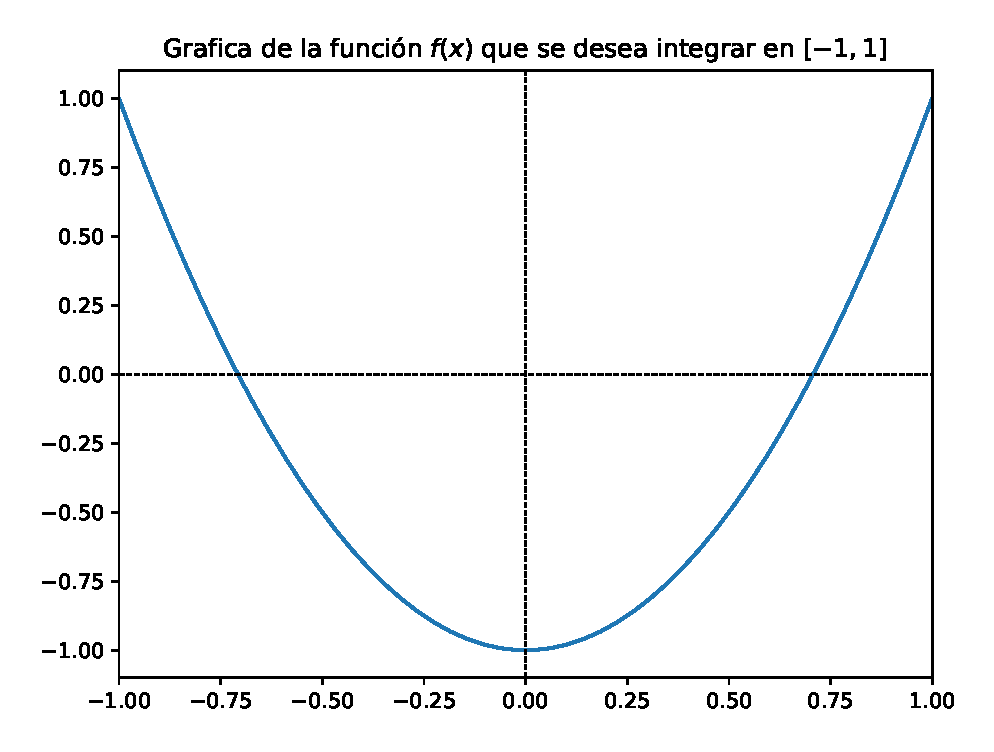
\includegraphics[scale=0.5]{Imagenes/integral_1_3_simpson.eps}
    \caption{Queremos calcular el valor del área debajo de la curva.}
\end{figure}
\end{frame}
\begin{frame}[allowframebreaks, fragile]
\begin{lstlisting}[caption=Propuesta de código, style=FormattedNumber, basicstyle=\linespread{1.1}\ttfamily=\small, columns=fullflexible]
def Simpson_13_(f, x_0_, xf, n):
   
   n = n - n%2 # truncar al numero par mas cercano
   print ('Para n= ' + str(n))
   
   if n <= 0:
      n = 1
   
   h = (xf - x_0_)/n
   x = x_0_
   
   suma = 0
   
   for j in range(int(n/2)):
      suma += f(x) + 4. * f(x + h) + f(x + 2 * h)
      x += 2 * h
   return (h/3.) * suma
\end{lstlisting}
\end{frame}
\begin{frame}[allowframebreaks, fragile]
\begin{lstlisting}[caption=Solución al problema, style=FormattedNumber, basicstyle=\linespread{1.1}\ttfamily=\small, columns=fullflexible]
def f(x):
    return cos(2 * acos(x))

for i in range(1, 4):
    print ('La integral I vale = ' + str(Simpson_13_(f, -1., 1., i * 2)) + '\n')
\end{lstlisting}
\end{frame}
\begin{frame}[fragile]
\frametitle{Solución en la terminal}
\begin{verbatim}
Para n = 2
La integral I vale = -0.6666666666666666

Para n = 4
La integral I vale = -0.6666666666666665

Para n = 6
La integral I vale = -0.6666666666666667 
\end{verbatim}
\end{frame}
\end{document}